\section{Implementarea DVM versiunea 2}

Implementarea simulatorului \gls{dvm} versiunea 2 folosește memoria internă și un fişier aflat în sistemul local de fişiere pentru stocarea și întoarcerea valorilor atributelor modelelor \gls{yang} pe care le expune. Fişierul de configurare conţine valori pentru toţi aceşti parametri și are o structură asemănătoare unui răspuns la operaţia \textit{get} al unui server \gls{netconf}. Această abordare este foarte avantajoasă, din două motive. În primul rând, dacă un dezvoltator de aplicații software \gls{sdn} are nevoie de alte valori pentru orice atribut \gls{yang}, este suficient să modifice acea valoare în fişier și să repornească simulatorul \gls{dvm}, fără a fi nevoie să cunoască detaliile de implementare sau să recompileze serverul \gls{netconf}. În cel de-al doilea rând, \gls{dvm} poate oferi răspunsuri similare cu un mediator real dacă în fişierul de configurare se va introduce răspunsul \gls{xml} venit de la un astfel de mediator la o operaţie \textit{get}.

Fluxul de lucru pentru operaţiile de aducere a atributelor este ilustrat în Figura \ref{fig:dvm_v02_workflow}.

\begin{figure}[h]
	\centering
	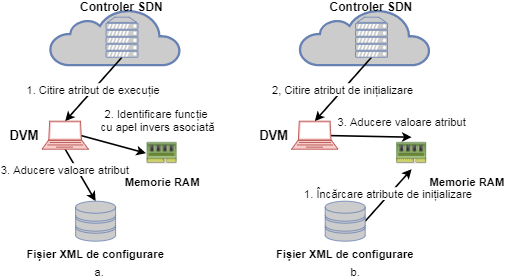
\includegraphics[width=1\textwidth]{dvm_v02_workflow}
	\caption{Fluxul de lucru pentru aducerea atributelor: a) de execuţie; b) de iniţializare \cite{stancu2017enabling}.}
	\label{fig:dvm_v02_workflow}
\end{figure}

Echipamentul de control \gls{sdn} care se conectează la simulatorul \gls{dvm} poate efectua diferite operații asupra parametrilor de execuţie sau de iniţializare. Acesta asigură funcţionalitatea necesară prin intermediul funcţiilor cu apel invers generice care se află în implementările nodurilor \textit{OpenYuma} pentru fiecare atribut, care vor evalua pentru ce parametru a fost invocată funcţia prin numele atributului. De exemplu, dacă echipamentul de control \gls{sdn} folosește o operaţie \gls{netconf} \textit{get} pentru a afla valoarea atributului de stare \textit{txFrequency} (frecvenţa emiţătorului), funcţia cu apel invers generică, asociată parametrilor de execuţie va fi invocată, va determina din numele parametrului că se doreşte valoarea pentru atributul respectiv și va întoarce valoarea corespunzătoare din fişierul \gls{xml} de configurare. Același lucru se întâmplă și pentru atributele de iniţializare, cu diferenţa că valoarea acestora va fi deja încărcată în memoria serverului \gls{netconf} din momentul inițializării simulatorului. Continuând exemplul anterior, dacă echipamentul de control are nevoie de valoarea parametrului \textit{txFrequencyMin} (valoarea minimă pe care frecvenţa emiţătorului o poate avea), o va întoarce din memoria aplicaţiei, deoarece în momentul inițializării \gls{dvm} aceasta a fost încărcată acolo de funcţia cu apel invers generică asociată atributelor de iniţializare.

Un caz special este reprezentat de atributele care sunt membre în liste. În această categorie se pot încadra, de exemplu, alarmele de pe dispozitiv, sau valorile indicatorilor de performanţă. Fiind parte dintr-o listă, există o valoare cheie care diferențiază intrările din listă. Aceasta este necesară în momentul în care se doreşte aflarea valorii unui astfel de atribut. Din această cauză, în momentul invocării funcţiilor cu apel invers generice pentru un parametru dintr-o listă, aceasta va trebui întâi să valideze cheia ca fiind parte din intrările din lista respectivă și abia apoi să apeleze funcţia asociată nodului respectiv.

Modelele \gls{yang} implementate în cea de-a treia demonstrație de concept \gls{onf} \cite{onf2016_poc3}, care au fost expuse și de simulatorul \gls{dvm} sunt parte din TR-532 și TR-512.1: \textit{MicrowaveModel-ObjectClasses-AirInterface}, \textit{MicrowaveModel-ObjectClasses-PureEthernetStructure}, \textit{MicrowaveModel-ObjectClasses-EthernetContainer}, \textit{CoreModel-CoreNetworkModule-ObjectClasses} și \textit{MicrowaveModel-Notifications}. Fiecare dintre acestea a fost transformat într-un modul al serverului \gls{netconf}, mai exact într-o bibliotecă partajată care să poată fi încărcată de codul de bază al serverului, existând o relaţie de 1:1 între un model \gls{yang} și un modul al serverului. Codul în limbajul C al simulatorului \gls{dvm} folosit în cea de-a treia demonstraţie de concept este de asemenea cu sursă deschisă și poate fi găsit în repertoriul \gls{onf} de pe platforma GitHub \cite{dvmv02github}.

În implementare a fost aplicat același principiu ca în prima versiune a \gls{dvm}: în funcțiile de iniţializare ale fiecărui modul a fost construită baza de stocare de date de execuţie arborescentă, folosind valorile cuprinse în fişierul \gls{xml} de configurare. Pentru implementarea diferitelor tipuri de parametri \gls{yang} (de iniţializare, de execuţie și de configurare) în \gls{dvm} a fost construită o bibliotecă statică, tot în limbajul C: \textit{\textbf{Base\_mediator\_utils}}. Printre fişierele mai importante pe care aceasta le cuprinde se numără, după cum este descris și în \cite{stancu2017enabling}:
\begin{itemize}
	\item \textit{boot\_time\_callbacks.c} - acest fişier expune o funcție cu apel invers generică, care este folosită în modulele serverului pentru a găsi valoarea atributelor \gls{yang} de iniţializare în fişierul de configurare \gls{xml}. Mai conţine de asemenea și funcții folosite pentru găsirea cheilor în cazul elementelor de tip listă care sunt prezente în model. Este nevoie de acestea în etapa de iniţializare, pentru a şti câte elemente sunt conţinute în listele respective. Intern (adică fără a fi expuse), acest fişier conţine câte o funcție asociată fiecărui parametru de iniţializare, a cărei implementare găseşte valoarea în fişierul \gls{xml} pentru atributul respectiv, însă nu direct, ci prin apelarea altor funcții, din raţiuni de lizibilitatea a codului;
	
	\item \textit{runtime\_callbacks.c} - acest fişier este asemănător cu cel anterior, diferenţa fiind făcută de atributele \gls{yang} pe care le referă. Astfel, în acest caz este vorba de atributele dinamice, de execuţie;
	
	\item \textit{configuration\_callbacks.c} - acest fişier sursă expune o funcție generică folosită pentru a seta valoarea unui atribut de configurare în fişierul \gls{xml} asociat. Aceasta este invocată în momentul folosirii unei operații de tip \textit{edit-config} de către un client \gls{netconf} (de exemplu echipamentul de control \gls{sdn});
	
	\item \textit{dvm\_boot\_time\_callbacks.c} - acest fişier a fost creat pentru îmbunătăţirea lizibilităţii codului și conţine implementările funcţiilor care citesc valoarea atributelor de iniţializare din fişierul \gls{xml};
	
	\item \textit{dvm\_runtime\_callbacks.c} - acest fişier are același rol cu cel anterior, cu diferenţa că referă atributele de execuție;
	
	\item \textit{utils.c} - acest fişier conţine funcții utilitare de care are nevoie biblioteca, cum ar fi funcții pentru citirea din fişierul de configurare sau funcții pentru crearea de noduri \textit{OpenYuma} în baza de stocare de date de execuţie.
\end{itemize}

Fiecare dintre bibliotecile partajate care corespund modelelor \gls{yang} sunt legate static de biblioteca \textit{\textbf{Base\_mediator\_utils}}. În acest mod se asigură o separare între logica de construire a bazei de stocare de date de execuţie a serverului \gls{netconf} și găsirea valorii atributelor \gls{yang} în fişierul \gls{xml} de configurare. Este un avantaj important al proiectării \gls{dvm}, deoarece oferă flexibilitate și posibilitatea de a înlocui uşor citirea valorilor din fişierul de configurare cu citirea acestora dintr-un echipament real de rețea, transformând simulatorul într-un mediator real, fără a fi nevoie de cunoașterea detaliilor de construire a bazei de stocare de date de execuţie.

Au fost considerate două abordări pentru citirea valorilor din fişierul de configurare \gls{xml}: o abordare dinamică și una statică. În abordarea dinamică, în momentul în care o funcție cu apel invers asociată unui atribut \gls{yang} dinamic este invocată, fişierul \gls{xml} este deschis, încărcat în memorie, valoarea respectivă este citită, apoi fişierul este scos din memorie și închis. Scopul acestei abordări era de a simula aspectul dinamic al parametrilor de stare. În cazul în care, între două citiri succesive, valoarea atributelor este schimbată în fişierul de configurare, acest lucru se va reflecta și în valorile trimise către echipamentul de control \gls{sdn}. Abordarea statică este reprezentată de încărcarea fişierului \gls{xml} în memorie în momentul primei invocări a funcţiei cu apel invers și citirea valorii atributului. Apoi, la următoarele citiri, fişierul de configurare va fi deja încărcat în memorie și valorile parametrilor vor fi întoarse de acolo. Astfel, datele vor fi statice, însă va fi nevoie de o singură citire de pe disc. În procesul de implementare, a fost evaluat timpul necesar citirii de pe disc, iar deoarece acesta era foarte mare în momentul în care se doreau valorile pentru mai multe atribute de execuţie, făcând timpul de răspuns al simulatorului extrem de mare, abordarea dinamică nu este prezentă în implementarea finală a simulatorului.

Generarea notificărilor \gls{netconf} este similară cu implementarea din prima versiune a simulatorului \gls{dvm}. În funcţia de iniţializare a modulului asociat modelului \gls{yang} care descrie notificările se crează un nou fir de execuţie care va genera notificări fictive. Conţinutul acestora va fi însă dinamic, nu static precum în versiunea anterioară. Detaliile notificării, dar și intervalul de timp dintre două notificări consecutive, vor fi citite din fişierul \gls{xml} de configurare. Cea de-a doua versiune a simulatorului \gls{dvm} oferă posibilitatea de a genera două tipuri de notificări, în funcție de conţinutul fişierului de configurare: \textit{attributeValueChangedNotification} (notificare care apare în momentul în care valoarea unui atribut se schimbă) și \textit{problemNoficitation} (reprezintă alarme care sunt generate de către dispozitiv).

A doua versiune a simulatorului \gls{dvm} oferă o implementare mai flexibilă și mai robustă față de prima versiune. Dacă în versiunea anterioară doar două atribute erau prezente în fişierul de configurare, orice modificare a altui parametru necesitând recompilarea simulatorului, acum \gls{dvm} le conţine pe toate în fişierul \gls{xml}, oferind posibilitatea dezvoltatorilor de aplicații \gls{sdn} de a modifica în mod facil aceste valori care vor fi interogate de către echipamentul de control. \gls{dvm} versiunea 2 expune modelele TR-532 și TR-512.1 în întregime \cite{stancu2017enabling}, nu doar un model simplificat, precum prima versiune. Și mecanismul de generare a notificărilor \gls{netconf} a fost îmbunătăţit, deoarece detaliile acestora pot fi modificare acum în fişierul de configurare.